%Results
\subsection{Stopping Probability as a Function of Round and Margin}
For both SO and EoR \BRAVO simulations, our software estimated round sizes that would give $\chi_j(\mathcal{A}) = 0.9$ and used those for the simulations. In Figure \ref{fig:eor_bravo_sprob}, we display the proportion of EoR \BRAVO audits that stopped in the $j^{th}$ round
to all audits which had not stopped before the $j^{th}$ round, for $j=1,2,3$. Though we carried out the simulations for $5$ rounds we show only the first three rounds of the simulations because very few audits, $(.1)^{j-1}\cdot(10^4)$ on average, 
make it to the $j^{th}$ round for $j \geq 4$. In Figure \ref{fig:so_bravo_sprob}, we display the same proportions for SO \BRAVO audits. 
In both cases, these proportions are estimates of the true value of $\chi_j(\mathcal{A})$ for $j=1,2,3$ as a function of margin. 
We see that, especially in earlier rounds for which 
the values are more representative of true audit behavior because fewer simulated audits have stopped, 
our round size predictions are accurate (the proportions are close to $0.9$).

\begin{figure}
\begin{centering}
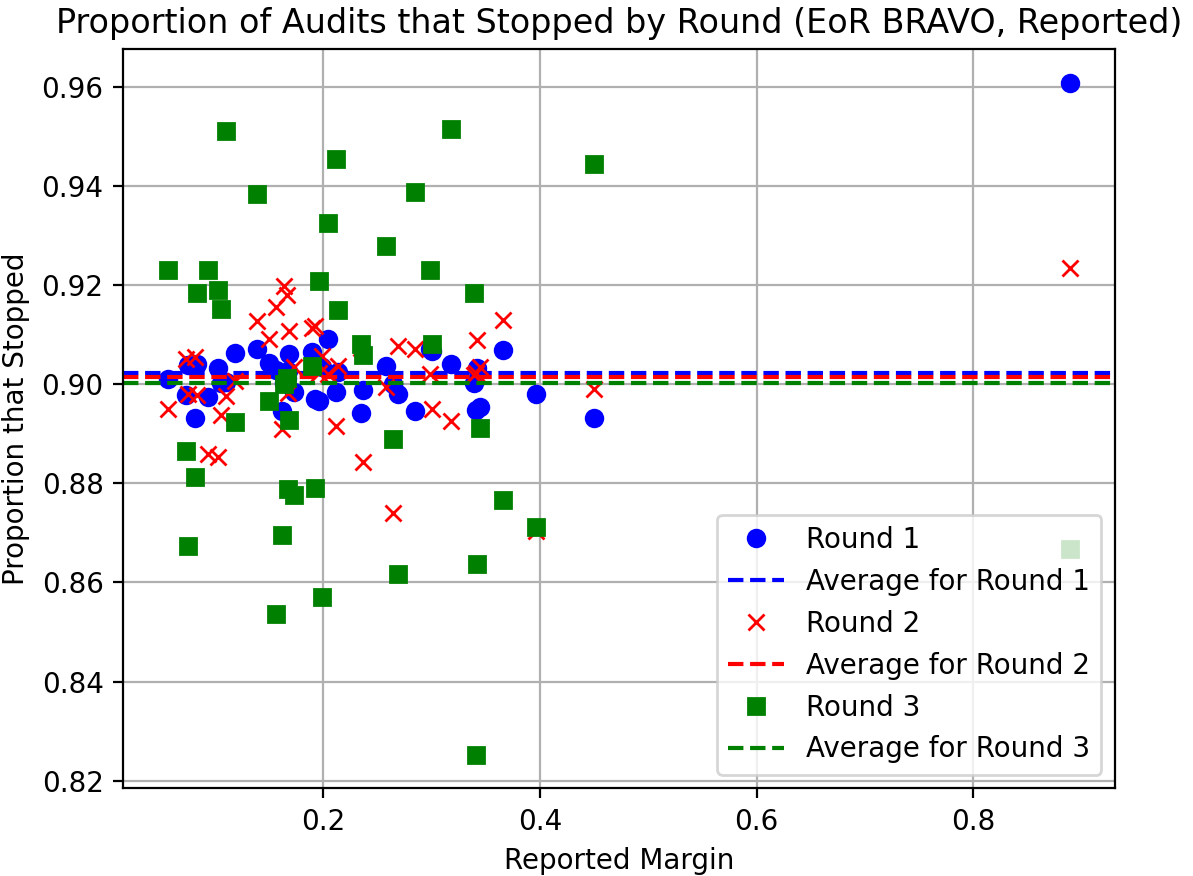
\includegraphics[width=0.8\textwidth]{eor_bravo_90perc_10^4_corrected/sprob_first_three_cropped.png}\caption{
This plot shows, for each state margin, when the underlying election is as announced, the number of EoR \BRAVO audits that stopped in the $j^{th}$ round,
as a fraction of all EoR \BRAVO audits which had not yet stopped before the $j^{th}$ round for $j=1,2,3$ and $S_1=0.9$.}
\label{fig:eor_bravo_sprob}
\end{centering}
\end{figure}

\begin{figure}
\begin{centering}
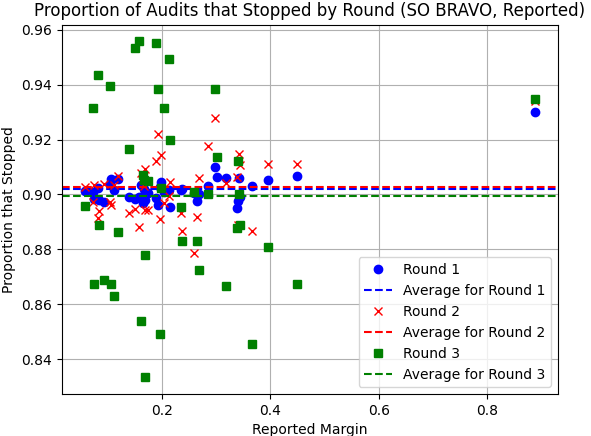
\includegraphics[width=0.8\textwidth]{so_bravo_90perc_10^4/sprob_first_three.png}\caption{
This plot shows, for each state margin, when the underlying election is as announced, the number of SO \BRAVO audits that stopped in the $j^{th}$ round,
as a fraction of all EoR \BRAVO audits which had not yet stopped before the $j^{th}$ round for $j=1,2,3$ and $S_1=0.9$.}
\label{fig:so_bravo_sprob}
\end{centering}
\end{figure}

Figure~\ref{fig:minerva1_sprob} and Figure~\ref{fig:minerva1p5_sprob} show the same proportions for \Minerva round multipliers of $1.0$ and $1.5$ respectively. We see that the first round size estimates were fairly accurate, with first round stopping probabilities being very close to $.9$. For subsequent rounds, the multipliers of $1.0$ achieved smaller stopping probabilities, as it was not chosen so as to obtain $\chi_j({\mathcal A}) = 0.9$. The $1.5$ multiplier is a good estimate for $j=2$, but the stopping probability for $j=3$ is slightly smaller than $0.9$. Note that we chose a simple multiplier for future rounds, but one could make more accurate round size estimates before the audit begins. 

\begin{figure}
\begin{centering}
\includegraphics[width=0.8\textwidth]{minerva_multiround_1x_10^4/sprobs_first_three.png}
\caption{This plot shows, for each state margin, when the underlying election is as announced, the number of \Minerva audits that stopped in the $j^{th}$ round,
as a fraction of all \Minerva audits which had not yet stopped before the $j^{th}$ round for $j=1,2,3$, round size multiple of $1.0$ and $S_1=0.9$.}
\label{fig:minerva1_sprob}
\end{centering}
\end{figure}

\begin{figure}
\begin{centering}
\includegraphics[width=0.8\textwidth]{minerva_multiround_1p5x_10^4/sprobs_first_three.png}
\caption{This plot shows, for each state margin, when the underlying election is as announced, the number of \Minerva audits that stopped in the $j^{th}$ round,
as a fraction of all \Minerva audits which had not yet stopped before the $j^{th}$ round for $j=1,2,3$, round size multiple of $1.5$ and $S_1=0.9$.}
\label{fig:minerva1p5_sprob}
\end{centering}
\end{figure}

Finally, we can perform a similar study for $S_1=0.25$. See \ref{fig:minerva_25} for an example, \Minerva with round mutiplier $1.5$. 

\begin{figure}
\begin{centering}
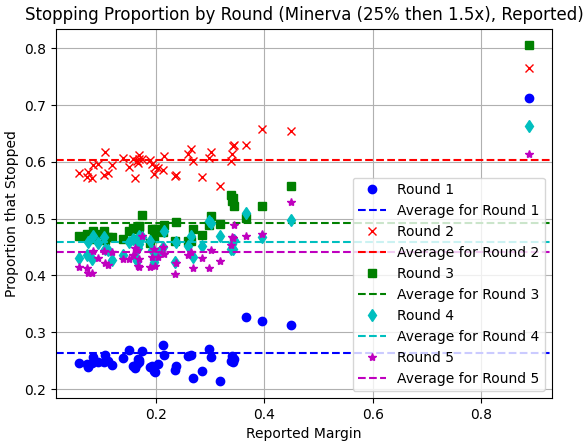
\includegraphics[width=0.8\textwidth]{minerva25percthen1p5_sprob.png}
\caption{This plot shows, for each state margin, when the underlying election is as announced, the number of \Minerva audits that stopped in the $j^{th}$ round,
as a fraction of all \Minerva audits which had not yet stopped before the $j^{th}$ round for $j=1,2,3$, round size multiple of $1.5$ and $S_1 = 0.25$.}
\label{fig:minerva_25}
\end{centering}
\end{figure}
\subsection{Maximum Risk as a Function of Round and Margin}
We also study the proportion of audits that stopped when the underlying election was a tie.
This proportion should approach a value less than the risk limit, $0.1$, as more audits are performed.

%\begin{figure}
%\includegraphics[width=0.8\textwidth]{eor_bravo_90perc_10^4_corrected/total_risk.png}
%\caption{This plot shows, for each state margin,
%the fraction of EoR \BRAVO audits that stopped in any of the $5$ rounds when the underlying election was a tie.}
%\label{fig:eor_bravo_risk}
%\end{figure}

\begin{figure}
\begin{centering}
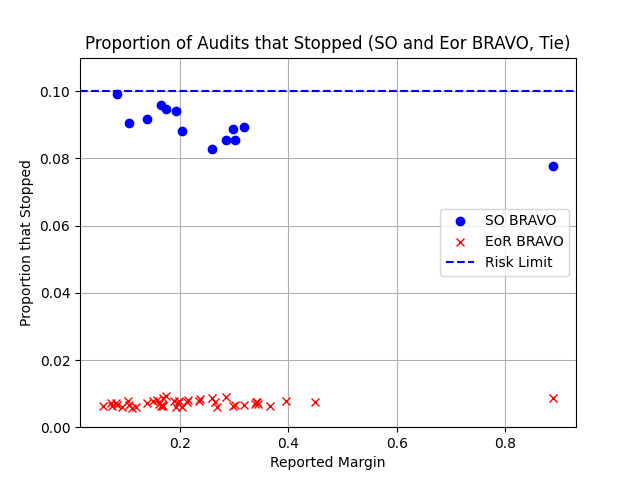
\includegraphics[width=0.6\textwidth]{bravo_risks_same_plot.png}
\caption{This plot shows the fraction of EoR \BRAVO audits (all states with margins at least $0.05$) and SO \BRAVO audits (the 13 states for which our simulations are complete so far) that stopped in any of the $5$ rounds when the underlying election was a tie.}
\label{fig:bravo_risk}
\end{centering}
\end{figure}

We observe that the risk of EoR \BRAVO is roughly
an order of magnitude less than the risk limit. 
These results are as expected, because EoR \BRAVO is known to be too conservative \cite{usenix_minerva}.  

In Figure~\ref{fig:bravo_risk} we show only the results for the $13$
states for which our simulations with an underlying tied election have completed.
To estimate the next round size that achieves a desired stopping probability,
the SO \BRAVO software generates the probability distribution on the number of ballots in the sample ballot by ballot (see \cite{usenix_minerva}) since
the stopping condition needs to be evaluated for each individual ballot drawn.
Because the underlying tied election causes audits to move on to larger rounds, 
the simulations are computationally expensive. SO \BRAVO is proven to be a Risk-Limiting Audit,
and we observe in Figure~\ref{fig:bravo_risk},
that the risk of SO \BRAVO is much
nearer the risk limit than that of EoR \BRAVO, as expected. 

%\begin{figure}
%\includegraphics[width=0.8\textwidth]{so_bravo_90perc_10^4/total_risk.png}
%\caption{This plot shows, for each state margin,
%the fraction of SO \BRAVO audits that stopped in any of the $5$ rounds when the underlying election was a tie.}
%\label{fig:so_bravo_risk}
%\end{figure}

%TODO SO and EoR macros

Figure~\ref{fig:minerva1p5_risk} show that fewer than $0.1$ of the audits stopped when the underlying election was a tie, for round multiples $1.5$, as would be expected for an RLA with risk limit $0.1$. 
Unlike EOR \BRAVO, the experimental risks here are much closer to the risk limit,
showing that \Minerva stops on average with a less conservative risk; \Minerva is sharper. The plot for round multiple $1.0$ is very similar. 

%\begin{figure}
%\begin{centering}
%\includegraphics[width=0.6\textwidth]{minerva_multiround_1x_10^4/total_risk.png}
%\caption{This plot shows, for each state margin,
%the fraction of \Minerva audits with a round size multiple of $1.0$ that stopped in any of the $5$ rounds when the underlying election was a tie.}
%\label{fig:minerva1_risk}
%\end{centering}
%\end{figure}

%For the Minerva simulations with a round size multiple of $1.5$,
%we increased the number of simulations to $10^6$ per state for 
%both an underlying tie and underlying announced outcome. 

%\includegraphics[width=\textwidth]{minerva_multiround_1p5x_10^6/total_risk.png}

% we could suggest that predicting accurate multiples is possible (same curve rather than line)

\begin{figure}
\begin{centering}
\includegraphics[width=0.6\textwidth]{minerva_multiround_1p5x_10^4/total_risk.png}
\caption{This plot shows, for each state margin,
the fraction of \Minerva audits with a round size multiple of $1.5$ that stopped in any of the $5$ rounds when the underlying election was a tie.}
\label{fig:minerva1p5_risk}
\end{centering}
\end{figure}




